\section{Implementation}
\label{sec:implementation}

The \SystemName-Lite system relies on two libraries that we implemented. First, we discuss the \texttt{pre} library\footnote{\url{https://github.com/etclab/pre}},
which implements the AFGH proxy re-encryption scheme in Go.~\cite{05-ndss-improved_proxy_reencryption}
Then we discuss the \texttt{samba} library\footnote{\url{https://github.com/etclab/samba}}, which calls provides a simple interface for the \SystemName system, relying on the \texttt{pre} library to perform the cryptographic operations.
Finally, we cover the \SystemName-Lite system itself, which is contained as a separate entity within the \SystemName repository.

\subsection{Proxy Re-encryption Library}
\label{sec:PRE}
%
We implemented a library for proxy re-encryption (PRE) in Go based on the AFGH proxy re-encryption scheme~\cite{05-ndss-improved_proxy_reencryption}.
The four main functions of the library are 
\begin{enumerate}
	\item \texttt{Encrypt}, which encrypts a message with a public key,
	\item \texttt{GenerateReEncryptionKey}, which generates a re-encryption key from a private key and a public key.
	\item \texttt{ReEncrypt}, which re-encrypts a message with a re-encryption key.
	\item \texttt{Decrypt1}, which decrypts a message with a private key,
	\item \texttt{Decrypt2}, which decrypts a re-encrypted message with a private key.
\end{enumerate}

The plaintext of a proxy re-encryption scheme is a random element from the target group of a bilinear map.
We defined a \texttt{KdfGtToAes256} function that converts the \texttt{pre} "plaintext" an AES key.
The true plaintext message must be encrypted under that key, and sent alongside the AES key which is encrypted with the \texttt{Encrypt} function.

\subsection{\SystemName Library}

% proxy object
We defined a \texttt{Samba\-Proxy} struct that contains the public parameters, a map of function instances to their replicas, a map of instance keys, and a map of function leaders.
Its methods perform tasks such as registering public keys, sending messages, and generating re-encryption keys.
The \texttt{BootProxy} method initializes the proxy, generating the public parameters, and starting up an HTTP server both for receiving function requests from sender, and for instances to be able to register their public keys with the proxy.

% instance object
We defined a \texttt{Samba\-Instance} struct that represents an individual instance of a function.
Its methods perform tasks such as generating re-encryption keys, responding to messages from the proxy, and sending messages to the proxy.
The \texttt{BootInstance} method initializes the instance, requesting the public parameters from the proxy, generating the instance a public/private key-pair, and registering its public key with the proxy.
Then it starts up an HTTP server to receive messages from the proxy, which can be function messages or re-encryption key requests.

% serialization object
Some of the fields underlying the \texttt{pre} public and re-encryption key structs are private, so in order to send them over the network we have to serialize those fields.
To do so, we created corresponding structs for the serialized versions of the keys.
These structs have \texttt{Serialize} and \texttt{Deserialize} methods that convert between the serialized and de-serialized versions.

% SambaMessage
Samba messages themselves are defined by as a struct called \texttt{Samba\-Message}.
\begin{lstlisting}
type SambaMessage struct {
	Target        FunctionId
	WrappedKey1   Ciphertext1Serialized
	WrappedKey2   Ciphertext2Serialized
	IsReEncrypted bool
	Ciphertext    []byte
}
\end{lstlisting}

The \texttt{Target} field is the function ID of the target function, which is used by the proxy to look up the function's leader instance.
The \texttt{WrappedKey1} and \texttt{WrappedKey2} fields store the encrypted parameters that when decrypted and passed to \texttt{KdfGtToAes256} yield the AES key.
The \texttt{IsReEncrypted} field is a boolean that indicates whether the message has been re-encrypted or not, and its value determines if \texttt{WrappedKey1} or \texttt{WrappedKey2} is used.
The \texttt{Ciphertext} field is the actual ciphertext of the message, which is encrypted with the AES key.
We used Go's \texttt{json} library to marshal \texttt{Samba\-Message}s into JSON, to be sent as http requests.
The receiver then un-marshals them back into \texttt{Samba\-Message}s and processes them.

% SambaCrypto
We defined a \texttt{Samba\-Crypto} interface to wrap the logic of encrypting, re-encrypting, and decrypting true plaintext messages. 
\begin{lstlisting}
type SambaCrypto interface {
	Encrypt(
		pp *pre.PublicParams,
		pk any,
		plaintext []byte,
		functionId FunctionId
	) (*SambaMessage, error)

	Decrypt(
		pp *pre.PublicParams,
		sk any,
		m *SambaMessage
	) ([]byte, error)

	ReEncrypt(
		pp *pre.PublicParams,
		rk *pre.ReEncryptionKey,
		m *SambaMessage
	) (*SambaMessage, error)

	GenReEncryptionKey(
		pp *pre.PublicParams,
		sk *pre.SecretKey,
		req *ReEncryptionKeyRequest
	) (*ReEncryptionKeyMessage, error)
}
\end{lstlisting}
This interface is implemented by the \texttt{SambaPRE} struct, which is what \SystemName-Lite uses to perform the cryptographic operations.
The \texttt{SambaRSA} struct also implements this interface, and we discuss in \S\ref{sec:evaluation} how we use it to compare the performance of \SystemName-Lite with a na\"{i}ve RSA implementation.

These methods mainly wrap calls to the \texttt{pre} library, and perform the serialization tasks mentioned earlier. The \texttt{Decrypt} method also handles the case where the message has been re-encrypted, calling \texttt{Decrypt2} instead of \texttt{Decrypt1} when the \texttt{IsReEncrypted} field in the \texttt{SambaMessage} is true.

%% The \SystemName library exposes \texttt{En\-crypt}, \texttt{De\-crypt}, \texttt{Gen\-erate\-Re\-Encryption\-Key} and \texttt{ReEncrypt} methods.
%% \SystemName-Lite calls these methods to perform the necessary operations.
%% These methods perform some serialization and formatting tasks, as well as call similarly-named methods in the PRE library to perform the cryptographic tasks.
%% The \SystemName-Lite system itself contains four services that can be built and run to simulate the eventual fully-featured \SystemName system.


%% For proxy re-encryption, the ciphertext can be re-encrypted by a re-encryption key generated from the private key of the original recipient and the public key of the new recipient.
%% %
%% It is important to note that if the message is re-encrypted, a different decryption function must be used.
%% %
%% Both \texttt{Decrypt1} and \texttt{Decrypt2} are implemented in our PRE library, and there is a significant increase in latency for \texttt{Decrypt2}, which we'll discuss in \ref{sec:evaluation}
%% 

%% %
%% \SystemName defines a \texttt{SambaProxy} struct:
%% 
%% \begin{verbatim}
%% type SambaProxy struct {
%% 	pp                *pre.PublicParams
%% 	functionInstances map[FunctionId][]InstanceId
%% 	instanceKeys      map[InstanceId]InstanceKeys
%% 	functionLeaders   map[FunctionId]InstanceId
%% }
%% \end{verbatim}
%% 
%% The cloud provider plays the role of the \texttt{SambaProxy} in FaaS systems.
%% %
%% Individual function replicas, also called instances, can use the public parameters to generate their public-private keypair, and register their public key with the proxy.
%% %
%% The function instances map keeps track of what replicas belong to what function. Knative will be periodically polled to keep this updated.
%% %
%% The instance keys map keeps track of public keys and re-encryption keys for every instance known to \SystemName.
%% %
%% The proxy needs to maintain the function leaders map, since incoming requests will be encrypted to the leader instance of each function's set of replicas, so the proxy must request that re-encryption keys from the leader.
%% %
%% A multitude of methods are defined on this struct that handle instances' and clients' requests to set public keys, send messages, etc.
%% 
%% 
%% \SystemName also defines a \texttt{SambaInstance} struct representing an individual instance of a function:
%% 
%% \begin{verbatim}
%% type SambaInstance struct {
%% 	Id           InstanceId
%% 	KeyPair      *pre.KeyPair
%% 	PublicParams *pre.PublicParams
%% }
%% \end{verbatim}
%% 
%% It contains an RSA key-pair, generated from the public parameters maintained by the proxy, which it also stores upon receiving them.
%% %
%% Like for the proxy, we've defined methods for instances to perform the tasks required of them such as handling (decrypting and acting on) messages, generating re-encryption keys when requested, etc.
%% 

%
\subsection{\SystemName-Lite}

The \texttt{proxy} service boots a \texttt{SambaProxy} that runs an HTTP server exposing endpoints for registering keys, and sending messages. 

The \texttt{alice} and \texttt{bob} services boot \texttt{SambaInstances} that request the public parameters from the proxy, generate public/private key-pairs for themselves, and register their public key back with the proxy. 
Then, they launch HTTP servers to which the proxy will make requests to send messages and request re-encryption keys.
We arbitrarily set \texttt{alice} to be the leader, which the sender encrypts to.
\SystemName-Lite doesn't do any real load balancing, since this is a responsibility of the eventual cloud provider.
To simulate it, however, when running \SystemName-Lite you can toggle between Alice being able to handle requests and too busy to handle requests, to see requests send to either Alice or Bob, who decrypt and respond.
%% In the latter case, \texttt{proxy} requests a re-encryption key from \texttt{alice}, so that it can re-encrypt the message and send it to \texttt{bob}.
%% This re-encryption key between alice and bob only needs to be generated once per instance pair, the first time that a message must be re-encrypted from one instance to another.
%% This will be important to keep in mind when we explore the performance impact of the \SystemName operations in section~\ref{sec:evaluation}.

The \texttt{sender} service is a simple application that calls \texttt{samba\-.En\-crypt} to encrypt a message, then sends it as an HTTP request to the proxy and prints the response.
Running these services in the order listed achieves \SystemName-Lite's goal of demonstrating the control flow of the \SystemName system.

%% %
%% We will implement \SystemName within Oak and the
%% OpenFaaS~\footnote{\url{https://www.openfaas.com}} serverless platform.
%% %
%% For proxy re-encryption, we will explore integrating both bilinear
%% map~\cite{ 05-ndss-improved_proxy_reencryption} and post-quantum
%% lattice-based schemes~\cite{17-tops-fast_proxy_re_encryption}.
%% %
%% For aggregate signatures, we will use BLS
%% signatures~\cite{03-eurocrypt-aggregate_signatures_bilinear_maps,
%% 03-pkc-threshold_multi_blind_signatures}.


% [42] HelloRetail  Nordstrom. Hello, retail! https://github.com/ Nordstrom/hello-retail, 2018.
% [6] CodePipeline AWS. Aws-codepipeline-stepfunctions.  https://github.com/aws-samples/ aws-codepipeline-stepfunctions, 2018.
% [7] MapReduceAWS Lab. Lambda reference architecture for mapreduce. https://github.com/awslabs/ lambda-refarch-mapreduce, 2018.


%% \begin{figure}[t]
%%     \centering
%%     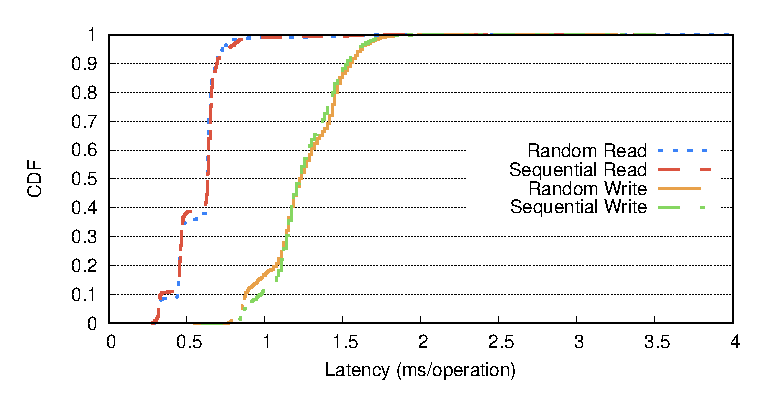
\includegraphics[width=0.5\textwidth]{figs/latency-cdf}
%%     %
%%     \caption{CDF of latencies for object read and write operations with \System (object size = 10M).}
%%     %
%%     \label{fig:latency-cdf}
%% \end{figure}
